\chapter{Charakterystyka środowisk}
\label{cha:charakterystyka_srodowisk}

Stworzenie autonomicznej, w pełni funkcjonalnej aplikacji wiąże się z wykorzystaniem wielu różnorodnych języków programowania, środowisk, baz danych i narzędzi. Odpowiednio szeroka wiedza na ich temat jest konieczna by móc w pełni skorzystać z ich potencjału. Inna kwestią jest umiejętne ich wybranie - tak by pasowały do potrzeb konkretnego projektu - oraz użycie, co niejako jest gwarantem ostatecznego sukcesu. Stąd też w kolejnych podrozdziałach pokrótce scharakteryzowane zostaną wszelkie udogodnienia, które zostały wykorzystane w celu implementacji nawigacji rowerowej. 

\section{Urządzenia mobilne z systemem iOS}

Od dłuższego czasu wyraźnie widać, że na rynku urządzeń mobilnych funkcjonują w zasadzie tylko dwa systemy operacyjne: Android oraz iOS. Zdecydowanie popularniejszy jest ten pierwszy, jednak i drugi ma niemałe grono oddanych użytkowników. iOS posiada jednak kilka atutów i niezaprzeczalnych zalet, które mocno odróżniają go od konkurenta. Przede wszystkim jest on w pełni zamkniętym systemem, którego twórca – amerykańska firma Apple – stworzyła bazując na własnym systemie operacyjnym Mac OS X. Ten ostatni powstał pod koniec XX wieku i napędzał komputery osobiste typu Macintosh. Oba te systemy bazują de facto na systemie Darwin, który z kolei ma Unixowy rodowód i jest oparty o jądro Mach, opracowane na amerykańskim Uniwersytecie Carnegie-Mellon. 
Sam system iOS zadebiutował wraz z premierą pierwszego iPhone'a, która odbyła się 9 stycznia 2007 roku na wystawie Macworld w San Francisco. Wówczas system ten był po prostu dostosowaną do realiów sprzętu mobilnego wersją systemu Mas OS X i nie posiadał własnej nazwy. Ta została nadana dopiero ponad rok później, w marcu 2008 roku i brzmiała iPhone OS. Po nieco ponad dwóch latach korporacja z Coupertino zdecydowała o jej skróceniu do formy iOS, która to nie zmieniła się już do czasu obecnego.
Jak wspomniano wcześniej system iOS jest systemem całkowicie zamkniętym i jedynym podmiotem, który oficjalnie mógł i może go modyfikować jest firma Apple, co z automatu powoduje, że jest ona również jedyną firmą, która może oferować sprzęt z preinstalowanym niniejszym systemem. Decyzja o wprowadzeniu takiej hermetyczności systemu miała swoje silne podwaliny w planach na firmowe portfolio produktów. Mianowicie amerykańska korporacja chciała wypuszczać na rynek pojedyncze urządzenia o konkretnej (w obrębie danej generacji) specyfikacji sprzętowej, dzięki czemu system można było bardzo mocno optymalizować. Plany zostały zrealizowane, a telefony czy też tablety z logo nadgryzionego jabłka stały się synonimem szybkości i stabilności działania, czego zdecydowanie nie można powiedzieć nawet o najdroższych urządzeniach z systemem Android.
System iOS złożony jest z 4 warstw abstrakcyjnych (logicznych): Core OS, Core Services, Media oraz Cocoa Touch. Najniższą jest Core OS, na którą składa się między innymi hybrydowe jądro Darwin, a jej rolą jest zapewnienie odpowiedniej interakcji między sprzętem a oprogramowaniem. Core Services jest zbiorem bazowych bibliotek, które zarządzają pracą wielu podstawowych funkcji,  niedostrzegalnych jednak bezpośrednio dla końcowego użytkownika, jak np. praca wątków i aplikacji, obsługa baz danych czy sieci. Za obsługę obrazu oraz dźwięku odpowiada warstwa Media, a w jej skład wchodzą między innymi biblioteki OpenGL czy Core Animation. Natomiast o poprawne działanie interfejsu użytkownika przy użyciu ekranu dotykowego dba warstwa Cocoa Touch. 

\section{Środowisko webowe}

Internet jest obecnie tak powszechnym medium, że wiele ludzi w ogóle nie wyobraża sobie bez niego codziennego funkcjonowania. Faktem jest, że jego popularyzacja ułatwiła dostęp do ogromnej bazy informacji (inną sprawą jest odpowiednie odsianie tych nieprawdziwych od prawdziwych) oraz komunikację między ludźmi. Jednak korzystacie z zasobów internetu nie byłoby możliwe – lub, co bliższe prawdzie, byłoby znacznie utrudnione – gdyby nie przeglądarki internetowe. Na rynku jest ich bardzo dużo, dostępne są na niemal każdy możliwy system operacyjny, a różnić się mogą zarówno wyglądem, funkcjonalnością, jak i silnikiem do renderowania stron. \newline
Najpopularniejszymi obecnie przeglądarkami na świecie są Google Chrome, Safari, Mozilla Firefox, UC Browser, Samsung Internet Browser, Opera, Internet Explorer oraz Edge. Zmianę ich rynkowego udziału w ostatniej dekadzie widać na obrazku Rys. 4.1.

\begin{figure}[H]
\centering
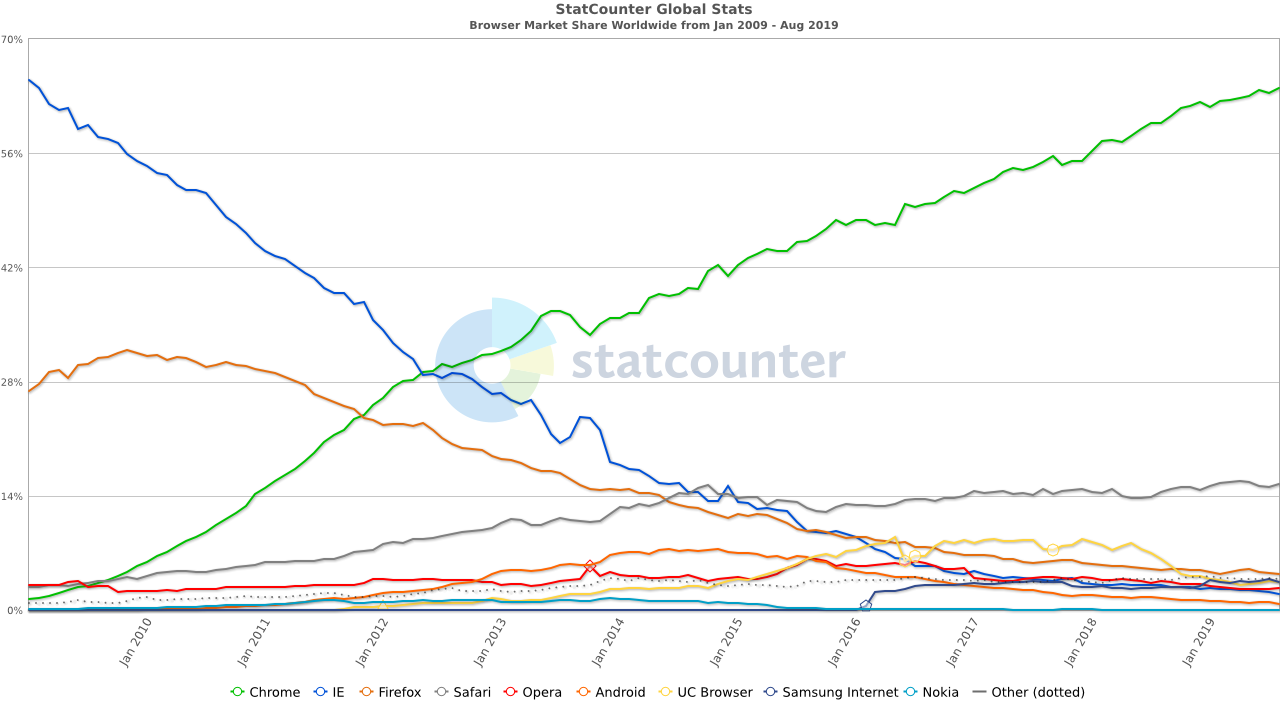
\includegraphics[width=\textwidth]{przegladarki_stats}
\caption{Statystyki użycia przeglądarek internetowych według witryny \protect\url{https://gs.statcounter.com/browser-market-share\#monthly-200901-201908} (stan na dzień 6.09.2019).}
\end{figure}

Jak widać Google Chrome mocno dominuje nad konkurencją, a pierwsze trzy przeglądarki mają w swych rękach ponad 80\% światowego rynku, dlatego też to właśnie one – jako te zdecydowanie najczęściej używane – zostaną poniżej pokrótce omówione.\newline
Google Chrome jest produktem firmy Google. Pierwsze jej wydanie miało miejsce 2 września 2008 roku i opierało się na rozwiązaniach open source po części bazując także na innych silnikach przeglądarek internetowych, między innymi na Mozilli czy WebKit'cie. Od wersji 28 wydanej w czerwcu i lipcu 2013 roku (w zależności od systemu) Chrome zaczął korzystać z własnego silnika Blink, opracowanego przez Google, a który jest forkiem komponentu WebCore silnika WebKit. Cechą charakterystyczną tej przeglądarki zawsze był minimalistyczny interfejs, a w początkach jej istnienia także rozdzielenie zakładek na osobne procesy, co wówczas było rozwiązaniem niespotykanym. Obecnie Google Chrome jest dostępny jako darmowa aplikacja na systemy Linux, Windows, macOS, Android oraz iOS.\newline
Drugą najpopularniejszą przeglądarką internetową jest produkt firmy Apple o nazwie Safari, której debiut odbył się 7 stycznia 2003 roku. Występowała ona wyłącznie na urządzeniach amerykańskiej firmy, poza okresem między rokiem 2007 a 2012, kiedy to dostępna była również wersja dla systemów Windows. Safari do renderowania stron korzysta z otwartego silnika WebKit, jednak pozostała część jej kodu (między innymi GUI) jest zamknięta, dostępna wyłącznie w formie binarnych plików wykonywalnych.\newline
Ostatnią z liczących się przeglądarek jest Mozilla Firefox autorstwa Mozilla Foundation. Jest to oprogramowanie o otwartym kodzie źródłowym wykorzystujące silnik Gecko, który również jest dziełem Mozilli. Jej pierwsze wydanie o numerze 0.1 datuje się na 23 września 2002 roku. Tym co wyróżniało Firefoxa na tle innych przeglądarek było łatwa możliwość modyfikacji, a co za tym idzie mnóstwo dostępnych dodatków, podzielonych na trzy kategorie: motywy, rozszerzenia oraz wtyczki. Program Mozilli był w zasadzie pierwszym, który udostępniał taką możliwość, czym rozpoczął modę na tego typu dodatkowe udogodnienia. Później podobne rozwiązania wprowadził między innymi Google Chrome czy Opera.

\section{Dane geoprzestrzenne}

Nie ma chyba ważniejszego aspektu w przypadku jakiejkolwiek aplikacji mającej na celu wyszukiwanie tras, niż dysponowanie odpowiednimi danymi obszaru, po którym chcemy nawigować. Oczywiście kluczowymi są dane geograficzne, ale zazwyczaj tego typu zbiory danych zawierają także wiele innych cennych informacji, stąd określa się je ogólnie jako dane geoprzestrzenne. Bazy tego typu danych są absolutnie niezbędne do stworzenia oprogramowania takiego rodzaju, jakiego podjęto się w niniejszej pracy.


\subsection{Dane urzędu miasta krakowa na temat ścieżek rowerowych (CartoDB)}

Głównym źródłem danych, którymi posiłkuje się stworzona aplikacja, są te na temat infrastruktury rowerowej miasta Krakowa autorstwa ZIKiTu. Dane te zebrane są w formie zbioru danych CartoDB. Jest on licencjonowany i dostarczany w tzw. modelu SaaS (z ang. Software as a Service) polegającym na subskrypcji centralnie hostowanej usługi. CartoDB idealnie nadaje się do przechowywania danych geoprzestrzennych, gdyż dokładnie w tym celu został zaprojektowany i stworzony. Opiera się on na relacyjnych bazach danych PsotgreSQL oraz PostGIS, która to dodaje do tej pierwszej obsługę danych geograficznych, dzięki czemu CartoDB obsługuje wiele formatów danych wejściowych. W realizacji projektu wykorzystano również język JavaScript (w części front-endowej aplikacji webowej) oraz Node.js (w bibliotekach oraz back-endowym API). Kreacja bazy danych przy pomocy CartoDB możliwa jest w sposób wizualny, to jest po prostu zaznaczając konkretne dane bezpośrednio na mapie. Jest to niewątpliwe sporą zaletą, gdyż ułatwia niedoświadczonym użytkownikom stworzenie bazy, a z drugiej strony także i wadą, gdyż powoduje takie problemy jak np. rozbieżność punktów sąsiadujących ze sobą elementów spowodowane zaznaczeniem minimalnie innych danych (rozdzielczość koordynat na mapie jest bardzo duża, więc nawet bardzo małe przesunięcie w miejscu na mapie, skutkuje innymi współrzędnymi geograficznymi).\newline
Same dane ZIKiTu obejmują swym zasięgiem jedynie gminę Kraków, lecz są całkiem obszerne i dokładne, choć rzadko aktualizowane. Poniżej można zobaczyć strukturę pojedynczego rekordy z niniejszej bazy na przykładzie Małego Rynku: \newline

\lstset{language=XML, breaklines=true}
\begin{lstlisting}
<Placemark>
<Style><LineStyle><color>ff0000ff</color></LineStyle><PolyStyle><fill>0</fill></PolyStyle></Style>
 <ExtendedData><SchemaData schemaUrl="\#infrastruktura_rowerowa_06_2018">
  <SimpleData name="cartodb_id">640</SimpleData>
  <SimpleData name="kategoria">c16t22-e</SimpleData>
  <SimpleData name="opis">Maly Rynek</SimpleData>
  <SimpleData name="dlugosc"></SimpleData>
  <SimpleData name="data"></SimpleData>
  <SimpleData name="szerokosc"></SimpleData>
  <SimpleData name="nawierzchnia">kostka brukowa</SimpleData>
  <SimpleData name="informacje_dodatkowe">kontraruch od Mikołajskiej do Siennej </SimpleData>
 </SchemaData></ExtendedData>
<MultiGeometry><LineString><coordinates>19.939853,50.060845 19.940441,50.06162 19.940424,50.061682</coordinates></LineString></MultiGeometry>
</Placemark>
\end{lstlisting}

Niestety można zauważyć pewien problem – a przynajmniej problem z punktu widzenia programisty chcącego stworzyć poprawny graf relacji opierając się na danych z niniejszej bazy – wynikający ze wspomnianego wcześniej graficznego tworzenia bazy. Otóż każda ulica czy ścieżka składa się w niej ze zbioru punktów, każdy określony współrzędnymi geograficznymi. Taki zbiór punktów nazywamy segmentem. Pierwszą niedogodnością jest fakt, że współrzędnego geograficzne punktów początkowych różnych segmentów w miejscu ich skrzyżowania delikatnie się od siebie różnią. W terenie różnice te sięgają co najwyżej kilku centymetrów, jednak od strony projektowej powodują konieczność wprowadzenia promienia wyszukiwania sąsiadujących punktów w momencie skrzyżowania się segmentów, gdyż bez tego nie dałoby się stworzyć spójnego grafu (precyzyjnie ujmując zawierałby on ledwie jeden segment – ten pierwszy, gdyż teoretycznie żaden segment nie byłby połączony z innym). Jednak powyższe zjawisko samo w sobie nie wydaje się nastręczać ogromnych problemów, zdecydowanie gorzej jest gdy dodamy do niego drugą wadę. Mianowicie punkty wchodzące w skład segmentu są definiowane tylko w przypadku, gdy segment, na który się składają, ulega zmianie kierunku w sensie geograficznym. Innymi słowy jeśli segment (czyli ulica lub ścieżka itp.) jest na jakimś swym odcinku poprowadzona idealnie na wprost, to baza zawiera jedynie punkt początkowy i końcowy takiego fragmentu. Oczywiście takie rozwiązanie jest sensowne i w normalnych przypadkach nie powoduje żadnych negatywnych konsekwencji. Jednak, jeżeli np. w połowie tego idealnie prostego fragmentu znajduje się skrzyżowanie z innym segmentem, to zbudowanie grafu relacji zaczyna być niemałym wyzwaniem. 

\subsection{Dane społeczności rowerowej (DaroPlan)}

Dane zebrane przez ZIKiT, choć dokładne i obszerne, okazały się niewystarczające by umożliwić silnikowi aplikacji znalezienie odpowiednich tras w każdym rejonie Krakowa. Dlatego też do projektu zdecydowano się dodać zbiór danych DaroPlan stworzony przez organizację pozarządową Otwarty Plan. Uzupełnia ona dane zgromadzone przez miejskich urzędników i powoduje, że na mapie Krakowa znacznie ubywa białych plam, czyli miejsc bez żadnych sugerowanych tras do przejazdu przy pomocy rowery. Zbiór ten również korzysta z CartoDB i został podobnie zdefiniowany.

\subsection{OpenStreetMap oraz Apple Maps}

OpenStreetMap jest otwartą mapą całej kuli ziemskiej tworzoną przez społeczność internetową. Jest ona całkowicie darmowa i swobodnie dostępna. Stworzył ją w 2004 roku Brytyjczyk Steve Coast, który inspirował się ogromną popularnością projektu Wikipedia. Coast pragnął by dane geograficzne również były ogólnodostępne, co w czasach sprzed powstania OpenStreetMap nie miało miejsca. Edytujący mapę muszą być zarejestrowani by móc wprowadzać zmiany, a w 2018 roku takich użytkowników było na świecie ponad 4.5 miliona. Dużym atutem mapy – poza jej darmowością i dostępnością – jest jej bardzo przyjazne API. Dzięki temu na przykład taki proces jak wyciągnięcie współrzędnych geograficznych danego adresu wiąże się z napisaniem prostego zapisania do bazy danych.\newline
Mapy Apple to usługa intenretowych map stowrzona przez Apple. Powstała ona dla systemów operacyjnych iOS, macOS i watchOS (w tej chronologii), a pierwsze wydanie miało miejsce 19 września 2012 i było wersja dla systemu iOS, zastępując funkcjonujące tam dotychczas Mapy Google. Apple Maps korzystają zarówno z danych opisanej wyżej OpenStreetMap, jak i z danych dostarczanych przez holenderską firmę TomTom. To co wyróżnia Mapy Apple na tle innych podobnych rozwiązań, to zastosowanie grafiki wektorowej do wizualizowania map. Taki sposób renderowania powoduje mniejsze zużycie danych oraz szybsze działanie mapy (a w zasadzie mniejszą zapotrzebowanie na zasoby sprzętowe).

\section{Użyte algorytmy}

Podstawowym problemem przy wszelkiego rodzaju aplikacjach wyznaczających trasy, jest problem najkrótszej ścieżki. W przypadku omawianego w niniejszej pracy zagadnienia wyszukiwania tras rowerowych, najbardziej reprezentatywnym matematycznym odzwierciedleniem danych o sieci ścieżek będzie graf, którego wierzchołki będą reprezentować skrzyżowania, a krawędzi odcinki pomiędzy nimi. Wagi tychże odcinków będą oznaczały ich długość. Z tego też powodu – rzeczywistego charakteru modelu – problem ten można zawęzić do poszukiwania najkrótszej ścieżki w grafie o wagach nieujemnych. Jest tak, ponieważ w rzeczywistości nie istnieją ścieżki, których długość wyraża się w liczbie ujemnej. W jaki sposób rozwiązać powyższy problem? Najbardziej logicznym rozwiązaniem, który pierwszy przychodzi do głowy jest zsumowanie wag wszystkich odcinków wchodzących w skład każdej możliwej tras z punktu startowego do końcowego i wybranie tej trasy, której sumaryczna waga jest najniższa. Jak łatwo się jednak domyślić, takie postępowanie jest niezwykle nieefektywne i w przypadku większej ilości odcinków oraz możliwych tras pomiędzy punktami początkowym i końcowym, zupełnie traci sens, gdyż jego złożoność obliczeniowa jest ogromna. Dlatego też istotnym jest wykorzystanie odpowiednich algorytmów działania, które pomogą w sposób efektywny (w stopniu większym lub mniejszym – w zależności od konkretnego algorytmu i problemu) rozwiązać problem znalezienia najkrótszej ścieżki w grafie o wagach nieujemnych.

\subsection{Algorytm Dijkstry}

Algorytm Dijkstry został wynaleziony w roku 1956 przez Edsgera W. Dijkstra. Jest jednym z najprostszych do implementacji sposobów wyszukiwania najkrótszych ścieżek w grafie, ale przy okazji jednym z najwolniejszych w działaniu. Umożliwia wyznaczenie ścieżek w grafie ważonym, w którym waga każdej z krawędzi jest nieujemna. Działanie algorytmu polega na przekazaniu punktu początkowego a następnie wyznaczeniu najkrótszych ścieżek do wszystkich innych wierzchołków inkrementacyjnie tworząc tablicę odkrytych ścieżek w każdym z odwiedzonych wierzchołków. W przypadku gdy nowo odkryta ścieżka nie jest jeszcze zapisana w tablicy ścieżek, zostaje do niej dodana. W przypadku gdy już tam istnieje, następuje sprawdzenie czy nowo odkryta ścieżka ma wagę mniejszą czy większą od już znalezionej. W przypadku znalezienia ścieżki o wadze mniejszej, obecnie istniejąca zostaje nią podmieniona, a algorytm kontynuuje działanie.\newline
Opisane działanie algorytmu powoduje że nie skaluje się on poprawnie w przypadku grafów o dużej ilości wierzchołków i krawędzi. Dzieje się tak ze względu na fakt że nie zawęża w żaden sposób obszaru swojego przeszukiwania. Złożoność obliczeniową grafu przedstawiono poniższym wzorem:\newline

\begin{equation}
O(|V|^2)
\end{equation}
gdzie
\begin{eqwhere}[2cm]
	\item[$V$] liczba wierzchołków w grafie 
\end{eqwhere}

Na podstawie przedstawionego wzoru możemy stwierdzić, że ilość obliczeń potrzebnych na wyznaczenie ścieżki rośnie eksponencjalnie wraz ze wzrostem ilości wierzchołków w badanym grafie.

\subsection{Algorytm A*}

Algorytm A* jest specjalną odmianą algorytmu Dijkstry, który wraz z przechodzeniem przez wierzchołki stara się optymalizować heurystykę przekazaną jako jeden z parametrów algorytmu. Przy przejściu przez każdy z wierzchołków, na podstawie informacji odnośnie poprzedniego i kolejnego przechodzonego wierzchołka, heurystyka wyznaczana jest na nowo co pozwala ominąć niektóre z nich. W przypadku gdy przekazana heurystyka jest stałą, algorytm wykazuje działanie identyczne do algorytmu Dijkstry. Z przekazanego opisu możemy odczytać że złożoność obliczeniowa algorytmu w znacznym stopniu zależy od złożoności obliczeniowej przekazanej heurystyki. Przykładowo w przypadku gdy wymaga ona iteracji po wszystkich wierzchołkach zawartych w grafie, wyznaczenie ścieżki staje się bardzo złożone. Algorytm A* jest szczególnie użyteczny w grafach posiadających swoje rzeczywiste odzwierciedlenie, jak na przykład mapę, w takim przypadku wyznaczenie heurystyki posiada liniową złożoność obliczeniową i uzyskany wynik jest bardzo dokładny.
W przeciwieństwie do algorytmu Dijkstra, algorytm A* umożliwia przeszukiwanie grafów nieskończonych, a także skaluje się dobrze dla grafów o bardzo dużej ilości wierzchołków i krawędzi. Algorytm kończy swoje działanie po odnalezieniu drogi którą uzna za optymalną, nie wymaga przeszukania reszty wierzchołków w przypadku wyspecyfikowania odpowiednio dokładnej funkcji heurystyki. Ogólną złożoność obliczeniową algorytmu A* przedstawiono poniższym wzorem:\newline

\begin{equation}
O((|V| + |E|) log |V|)
\end{equation}
gdzie
\begin{eqwhere}[2cm]
	\item[$V$] liczba wierzchołków w grafie 
	\item[$E$] liczba krawędzi w grafie 
\end{eqwhere}

W aplikacjach, w celach porównawczych, zaimplementowano jeszcze kilka innych metod wyznaczania najkrótszych ścieżek. Wszystkie jednak są pewnymi modyfikacjami algorytmu A*, a różnice zostały opisane podczas analizy.

\section{Metoda Haversine}

Metoda Haversine jest algorytmem służącym do wyznaczania odległości w linii prostej pomiędzy dwoma punktami znajdującymi się na sferze. W przypadku projektu będącego częścią tej pracy została wykorzystana do wyznaczania odległości pomiędzy punktami na mapie. Wyznaczone odległości zakładają pewną niedokładność, jako że ziemia nie jest idealną sferą. Jednak średni błąd wyznaczenia odległości przy użyciu metody Haversine jest tak mały że może zostać zignorowany przy założeniu skali długości wyznaczanych dróg mających zazwyczaj kilkaset lub więcej metrów długości.\newline
Obliczenia odległości sprowadzają się do rozwiązania równania (4.3)

\begin{equation}
d=2*r*arcsin*\sqrt{sin^2(\frac{\varphi_{2}-\varphi_{1}}{2}) + cos(\varphi)*cos(\varphi)*sin^2(\frac{\lambda_{2}-\lambda_{1}}{2})}
\end{equation}
gdzie
\begin{eqwhere}[2cm]
	\item[$d$] odległość
	\item[$r$] promień sfery
	\item[$\varphi_{1}$] szerokość geograficzna pierwszego z punktów 
	\item[$\varphi_{2}$]  szerokość geograficzna drugiego z punktów 
	\item[$\lambda_{1}$] długość geograficzna pierwszego z punktów 
	\item[$\lambda_{2}$] długość geograficzna drugiego z punktów
\end{eqwhere}

\section{Użyte języki programowania}

W celu stworzenia aplikacji serwerowej i strony www użyto szeregu bibliotek open-source. Ich zastosowanie pozwala na zdecydowaną redukcję ilości kodu potrzebnego w celu osiągnięcia oczekiwanego elementu. Każda z użytych bibliotek jest to osobna technologia, wymagająca użycia odrębnego języka programowania. W poniższych paragrafach opisano w skrócie wszystkie języki programowania oraz technologie użyte podczas pisania aplikacji będących elementem tej pracy.

\subsection{Język programowania JavaScript}

Javascript jest to skryptowy, wysoko poziomowy język programowania który jest aktualnie jednym z głównych języków programowania używanych przy pisaniu stron internetowych. Swoją popularności zyskał faktem, że aplikacje internetowe stworzone przy jego użyciu są renderowane po stronie klienta, nie serwera, co znacznie odciąża zasoby potrzebne do ich obsługi. Javascript bazuje na paradygmacie programowania funkcyjnego i imperatywnego.\newline
Od swojego powstania, w roku 1955, język bardzo ewoluował a z jego elastyczności korzysta wiele technologi często zupełnie nie związanych z tworzeniem interfejsów użytkownika w stronach internetowych. W obecnej chwili, wraz biblioteką Node.js oraz kilkoma mniej popularnymi, jest używany do pisania aplikacji serwerowych nastawionych głównie na szybkie reakcje i działanie w czasie rzeczywistym. W niedalekiej przeszłości znalazł nawet zastosowanie w pisaniu hybrydowych aplikacji mobilnych, w środowisku React Native, gdzie po napisaniu jest tłumaczony do kodu natywnego dla każdej z wybranych platform mobilnych.\newline
Jako ciekawostkę można przekazać, że język JavaScript, pomimo podobnej nazwy, nie ma nic wspólnego językiem programowania Java. Jego wypuszczenie na świat zbiegło się w czasie ze znaczną popularnością języka Java, a autorzy chcieli, nazywając go w ten sposób, sztucznie zwiększyć jego popularność.

\subsection{Język programowania Swift}

Język Swift jest funkcyjnym, statycznie typowym językiem programowania wypuszczonym przez firmę Apple w roku 2014 w celu zastąpienia przestarzałego języka Objective-C. Jest bardzo nowoczesnym językiem który od swojego początku co roku zdobywa nowe aktualizacje, często znacznie zmieniające jego działanie. Jest stworzony z myślą o pisaniu bezpiecznego kodu, który w czasie kompilacji będzie wykonywał znaczną ilość weryfikacji sprawdzających czy kod napisany przez użytkownika nie tylko będzie działał, ale także działał poprawnie. Jednym z przykładów tego zachowania są zmienne typu \textit{Optional} które przy poprawnym użyciu praktycznie uniemożliwiają odniesienie się do zmiennej która nie istnieje w pamięci i wywołania wyjątku null pointer. Język natychmiast po wprowadzeniu zgromadził wokół siebie ogromną ilość fanów, którzy zaczęli tworzyć rozszerzenia do oferowanych przez niego bibliotek oraz własne rozwiązania typu open-source.\newline
Swift został początkowo stworzony jako język do pisania aplikacji mobilnych na systemy operacyjne iOS oraz OS X dystrybuowane przez firmę Apple. Szybko jednak zdecydowano się na udostępnienie go jako open-source, oraz dodanie kompatybilności oraz kompilatora pod inne systemy bazujące na unix. Obecnie, poza tworzeniem aplikacji na urządzenia firmy Apple, Swift znalazł zastosowanie także jako biblioteka do tworzenia aplikacji internetowych korzystając przy tym z bibliotek takich jak \textit{Vapor} czy \textit{Kitura}.

\subsection{Biblioteka ReactJS}

Jedną z głównych bibliotek, używanych do tworzenia interfejsów użytkownika w aplikacjach internetowych jest biblioteka ReactJS. Jest to stosunkowo nowa technologia, wdrożona przez firmę Facebook w roku 2003. Po swojej premierze natychmiast zyskała wielu zwolenników a wiele firm zaczęło ją traktować jako główną technologię i przepisywać swoje istniejące rozwiązania. Przyczyną tego była prostota pisania kodu, stabilność i fakt zdecydowania się na obsługę jednego z najbardziej popularnych języków programowania w obecnym czasie. Biblioteka korzysta ze wszystkich standardowych funkcji języka Javascript do tworzenia logicznych części aplikacji, oraz wprowadza nowy standard deklaratywnego tworzenia interfejsów przy użyciu autorskiego rozwiązania - składni \textit{JSX}. \textit{JSX} umożliwia szybkie tworzenie widoku strony internetowej korzystając przy tym z predefiniowanych przez bibliotekę React elementów takich jak widok, tekst, tabela itp.. Stworzone aplikacje bazują na zmiennej aktualnego stanie - jest to zestaw zmiennych zdefiniowanych przez zmienną o nazwie \textit{state} w każdym z widoków. W przypadku zmiany któregokolwiek z elementów obiektu, następuje wywołanie metody render, która powoduje przeładowanie widoku. Renderowanie widoku jest możliwe dzięki React DOM. Jest to narzędzie które na podstawie przekazanego kodu JSX tworzy drzewo widoków obecnych w aktualnie wyświetlanym interfejsie, następnie przy każdej aktualizacji przelicza które z elementów powinny zostać zmienione aby poprawnie wyświetlić widok, dostosowując się do aktualnego stanu. Dzięki użyciu React DOM aplikacje stworzone przy użyciu ReactJS są bardzo wydajne.

\subsection{Biblioteka Node.js}

W celu implementacji aplikacji serwerowej użyto biblioteki Node.js, jest to stosunkowo nowa technologia, jej pierwsza wersja ujrzała światło dzienne w roku 2009. Node.js umożliwia wykonywanie kodu Javascript poza przeglądarką użytkownika, po stronie serwerowej, składa się z silnika V8 zaimplementowanego przez firmę Google oraz zestawu bibliotek dołączonych przez twórcę bilioteki w celu stworzenia wieloplatformowego środowiska do uruchamiania skryptów napisanych w kodzie Javascript. Biblioteka Node.js jest zaimplementowana w oparciu o architekturę \textit{event-driven} i asynchroniczne operacje wyjścia i wejścia, co oznacza, że biblioteka wydajnie wykorzystuje wielowątkowość i nie zostaje zablokowana wykonywaniem długich operacji przez równolegle działające procesy. Zważając na opisane wcześniej charakterystyki, oprogramowanie stworzone przy użyciu Node.js wyróżnia się dużą wydajnością oraz jest optymalnym wyborem dla aplikacji oczekujących szybkiego przetwarzania lub komunikacji w czasie rzeczywistym. Dodatkową zaletą biblioteki Node.js jest fakt, że wykorzystuje ten sam język programowania, którego używa się do programowania stron internetowych, z racji tego bariera wejścia do tworzenia pełnych systemów jest znacznie mniejsza.

\section{Użyte narzędzia}

W celu stworzenia aplikacji serwerowej oraz aplikacji mobilnej został użyty narzędzi programistycznych. Każda z użytych technologii korzysta z osobnego, często dedykowanego środowiska programistycznego, czyli aplikacji z wbudowanym edytorem tekstu przystosowanym do danego języka oraz debuggerem. Aby umożliwić sprawne tworzenie aplikacji w zespole użyto także odpowiednich aplikacji do testowania oraz systemu kontroli wersji. Wszystkie użyte przy tworzeniu oprogramowania technologie i narzędzia zostały opisane w poniższych paragrafach.

\subsection{Środowisko programistyczne Xcode}

Aplikacja na system iOS została stworzona przy użyciu środowiska programistycznego Xcode. Jest to rozbudowana aplikacja, opublikowana i rozwijana przez firmę Apple, głównie w celu tworzenia aplikacji pod systemy operacyjne iOS oraz OS X. Umożliwia jednak także kompilację języków C oraz C++ dzięki wbudowanym kompilatorom LLVM i GCC. W celu debugowania, środowisko używa debuggera LLDB, który w bardzo prosty, graficzny sposób przedstawia konsolę oraz umożliwia zatrzymanie egzekucji programu w danej linijce kodu, przechodzenie pomiędzy kolejnymi linijkami oraz cały zestaw zaawansowanych komend umożliwiających prezentację logów i egzekucję kodu implementowanego przez aplikację. Środowisko składa się z zaawansowanego edytora tekstu z wbudowaną obsługą składni języków Swift, Objective-C, C oraz C++. Poza standardową edycją podpowiadającą auto-uzupełnianie nawiasów i odpowiednie wcięcia, opisywane środowisko ma także wbudowany świetnie działający system auto-uzupełniania kodu. Jest to funkcjonalność niezmiernie przydatna jako że języki proponowane przez firmę Apple bazują na bardzo opisowej składni gdzie często jedna metoda jest długości nawet kilku linii kodu.\newline
Środowisko programistyczne Xcode ma także wbudowane system uruchomieniowy umożliwiający włączenie oprogramowania na realnym urządzeniu - komputerze lub telefonie. W przypadku braku realnego urządzenia z systemem iOS, możliwe jest także użycie symulatora dowolnego z urządzeń z dowolną wersją systemu operacyjnego. W celu instalacji aplikacji w systemie iOS na rzeczywistym urządzeniu jest jednak wymagane posiadanie opłacanego konta \textit{Apple Developer} oraz stworzenie w portalu odpowiednich certyfikatów.

\subsection{Narzędzie do testowania API Postman}

Aplikacja serwerowa udostępnia interfejs programistyczny umożliwiający dostęp do zasobów z zewnętrznych źródeł. Został stworzony w celu integracji aplikacji mobilnej. Aby umożliwić odpowiednie testowanie oraz wymianę danych testowych pomiędzy programistami pracującymi nad projektem użyto aplikacji Postman. Jest to prosta w użyciu aplikacja stworzona przez firmę Google w środowisku Electron. Umożliwia wykonywanie zapytań pod podany adres URL oraz daje interfejs graficzny do dodawania parametrów zapytania takich jak dane przesłane w zapytaniu lub nagłówki HTTP. \newline
W celu wymiany danych testowych pomiędzy osobami pracującymi nad projektem, występuje także możliwość eksportowania zestawu zdefiniowanych zapytań a następnie importowaniu ich w aplikacji u drugiej z osób.

\subsection{System kontroli wersji Git}

System git jest to rozproszony system kontroli wersji umożliwiający programistom jednoczesne tworzenie oprogramowania. Jest ono przetrzymywane w repozytorium, a dzięki mechanizmom rozgałęziania oraz ponownego scalania kodu umożliwia nawet jednoczesną edycję tych samych fragmentów kodu przez wiele osób. Poza systemem git istnieje na rynku kilka pokrewnych rozwiązań, jak na przykład system SVN, jednak w obecnej chwili git jest wiodącym oprogramowaniem z którego korzysta znaczna większość programistów i firm.\newline
Wszystkie części stworzonego systemu są przetrzymywane oraz synchronizowane przy użyciu systemu kontroli wersji git w witrynie \url{https://github.com}. Jest to jeden z najczęściej używanych hostingów do dystrybuowania aplikacji typu open-source. Dzieje się tak dzięki temu że konta nie posiadające prywatnych repozytoriów są całkowicie darmowe, niezależnie od ilości ludzi pracujących nad nimi.

